\section{\label{sec:nmp:systemwide}System-wide-synchronicity messaging}

\cpresetrulenumber

In this section, we present the first \gls{nmp} variant, wherein the entire system evolves as one, and every \gls{pe} executes the same rule(s) simultaneously.  For this paper, we assume that all \glspl{pe}, channels, the oracle, and environment behave correctly and follow their respective protocols, without faults, corruptions, lost messages, \textit{et cetera}.  This significantly simplifies the presented systems by allowing us to elide error handling concepts and describe only the intended operation.

\begin{figure}
    \centering
    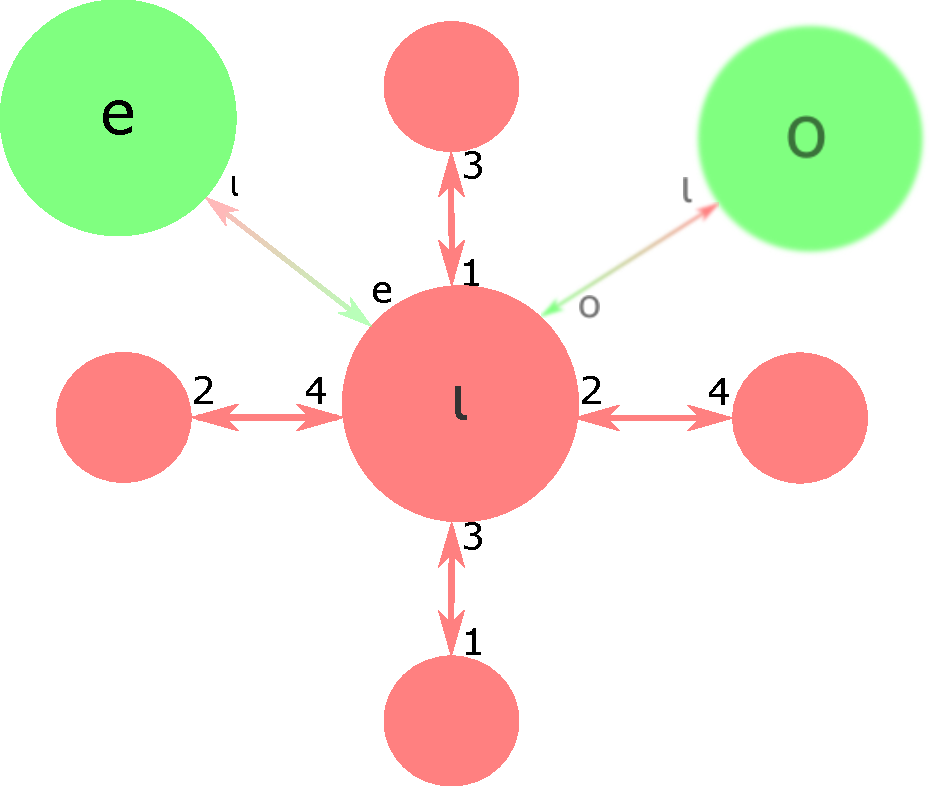
\includegraphics[width=0.9\textwidth]{chapters/nmp/images/iota_proxels_environment_oracle_v4.pdf}
    \caption[The communication topology of an \acrlong{nmp} system from the perspective of an arbitrary \acrshort{pe} in a \gls{fne} arrangement]{The communication topology of the system from the perspective of an arbitrary \gls{pe} in a \gls{fne} arrangement}
    \label{fig:nmp:iota_proxels_environment_oracle}
\end{figure}

The layout of the system, from the perspective of an arbitrary \gls{pe}, is depicted in \cref{fig:nmp:iota_proxels_environment_oracle}.  The central circle is said arbitrary \gls{pe} and is labelled with \(\iota\) to represent its ID in the overall system.  It is connected to each neighbour, the environment, and the oracle by two-way channels.  The neighbours themselves are anonymous, but \(\iota\)'s end of each channel is labelled with a number from 1-4, representing the neighbours who are expected to sit above, to the right, below and to the left of the central \gls{pe}, respectively.  The oracle is blurred in \cref{fig:nmp:iota_proxels_environment_oracle}, to reflect that it is a stand-in for an unspecified process that ordinarily would take place \emph{inside} the \gls{pe}.

In our approach, each \gls{pe} has \emph{no} direct knowledge of its neighbouring \glspl{pe}.  Instead, it interacts with channels that connect on the other end to those neighbours; the channels interpose between the \glspl{pe}.  Furthermore, each label for a neighbour in a given \gls{pe} is \emph{not} the system's ID for that neighbour, but the \gls{pe}'s label for a connecting channel endpoint.  Nevertheless, as a shortcut, we will refer to \glspl{pe} as simply communicating with their neighbours.  Messages exchanged by \glspl{pe} may be referred to as \emph{\acrfull{nm} messages}, while messages exchanged with the oracle may be referred to as \emph{\acrfull{oq} messages}.

In the synchronous version, the entire system evolves in lock-step, and thus is always in the same phase and \gls{cps} state.  This follows a basic process, consisting of four conceptually distinct phases, the middle two of which may be repeated.  Specifically, the system proceeds as follows:

\begin{enumerate}
    \item\label{enumitem:nmp:init} Initialisation (rules 1 \& 2)
    \item\label{enumitem:nmp:pu} \Gls{oq} (rules 4, 5 \& 6)
    \item\label{enumitem:nmp:nm} \Gls{nm} (rule 7)
    \item\label{enumitem:nmp:final} Finalisation (rules 3, 8 \& 9)
\end{enumerate}

This progression is depicted as a state machine in \cref{fig:nmp:systemwidestatemachine}.  State \(s_1\) covers the initialisation phase; \(s_2\) and \(s_3\) the \gls{oq} phase; \(s_4\) the \gls{nm} phase; and \(s_5\) and \(s_6\) the finalisation phase.  State \(s_7\) is the halting phase of the system's evolution.  In an application of \gls{nmp} phases \ref{enumitem:nmp:init}, \ref{enumitem:nmp:nm} and \ref{enumitem:nmp:final} will not change.  Only phase \ref{enumitem:nmp:pu} would be replaced.  The system's evolution is sketched at a high level in \cref{alg:nmp:systemwide2}.

\begin{figure}
    \centering
    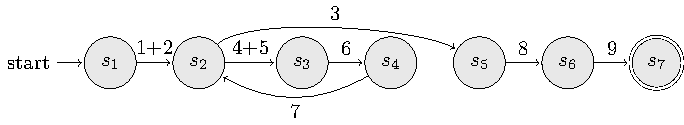
\includegraphics{chapters/nmp/images/systemwidestatemachine.pdf}
    \caption[State machine of the progression of the system-wide \acrlong{nmp} \gls{cps} rules.]{State machine of the progression of the system-wide \gls{nmp} \gls{cps} rules.  The vertices are labelled with states and the arcs with the rule(s) which cause the state transitions.}
    \label{fig:nmp:systemwidestatemachine}
\end{figure}

\begin{algorithm}
\DontPrintSemicolon
\KwOut{Final result, \(z\), sent to \(e\)}
\SetKwFor{pForEach}{parallel foreach}{do}{endfch}
\Begin{
    \tcc{\(a \Leftarrow \langle b \rangle\) denotes receiving object \(a\) on channel \(b\);\newline\(c \Rightarrow \langle d \rangle\) denotes sending object \(c\) on channel \(d\);\newline\(e \Leftrightarrow \langle f \rangle\) denotes antiport exchange, sending \emph{and} receiving (swapping) objects \(e\) on channel \(f\).}\;
    
    \tcc{Initialisation}
    \(i \Leftarrow \langle e \rangle\)\;
    \lpForEach{\((x,d) \Leftarrow \langle e \rangle\)}{\(v[x] \gets d\)}\;
    
    \While{i > 0 }{
        \tcc{\Glsentrylong{oq}}
        \(i \gets i - 1\)\;
        \pForEach{\(x \in \{1, 2, 3, 4\}\)}{
            \(w[x] \gets v[x]\)\;
            \(w[x] \Rightarrow \langle o \rangle\)
        }
        \lpForEach{\((x,d) \Leftarrow \langle o \rangle\)}{
            \(v[x] \gets d\)\
        }
        
        \;\tcc{\Glsentrylong{nm}}
        \lpForEach{\(x \in \{1, 2, 3, 4\}\)}{\(v[x] \Leftrightarrow \langle x \rangle\)}
    }
    \;\tcc{Finalisation}
    \pForEach{\(x \in \{1, 2, 3, 4\}\)}{
        \(w'[x] \gets v[x]\)\;
        \(w'[x] \Rightarrow \langle o \rangle\)
    }
    \(z \Leftarrow \langle o \rangle\)\;
    \(z \Rightarrow \langle e \rangle\)
}
\caption[Pseudocode of the \acrlong{nmp} process in the synchronous system]{\label{alg:nmp:systemwide2}Pseudocode description of the process for an individual \gls{pe} in the synchronous system}
\end{algorithm}

While we assume before the start of the system's evolution that the correct number of \glspl{pe} are already in place, they are all empty at the beginning of the system except for appropriate channel endpoints.  Everything else required by each \gls{pe} will be supplied by the environment or oracle, or generated by rules during the \gls{pe}'s evolution.  The rules for the synchronous system are listed in \cref{ruleset:nmp:systemwide} and explained below.  We first define the \gls{gs} \gls{nmp} system, explain the intended operation of the ruleset, then describe each of the ground terms used.

\subsection{System Definition}
Recall from \cref{sec:nmp:notation} that a given \gls{cps} implementation can be defined as a 6-tuple:
\[
\Pi_{cP}(T, A, O, R, S, \bar{s})
\]

\(T\) is a set of top-level cells, each representing a single \gls{pe}, numbered from one to the total size of the lattice.  These numbers correspond to the \(\iota\) of \cref{fig:nmp:iota_proxels_environment_oracle}.  \(A\) is the set of all terms defined in \cref{sec:nmp:systemwide:definitions}.  Each \gls{pe}'s starting multiset in \(O\) is empty barring appropriate channel endpoints.  Every \gls{pe}'s ruleset in \(R\) is equal to that in \cref{ruleset:nmp:systemwide}.  \(S = \{s_1, s_2, s_3, s_4, s_5, s_6, s_7\}\), i.e., the states defined in \cref{sec:nmp:systemwide:definitions}, and \(\bar{s} = s_1\) for all \glspl{pe}.

\subsection{Description of Rules}

\begin{cprulesetfloat}
    \begin{cpruleset}
        % Receive maximum generation counter
        \cprule{s_1}{\cprecv{\cpfunc{i}{I}}{e}}{1}{s_2}{\cpfunc{i}{I}}
        
        % Receive inputs from environment
        \cprule{s_1}{\cprecv{\cpvq{X}{D}}{e}}{+}{s_2}{\cpvq{X}{D}}
        
        \\
        
        % Else move to finishing
        \cprule{s_2}{i(\lambda)}{1}{s_5}{}
        
        % Decrement iterator
        \cprule{s_2}{i(I\cpundig)}{1}{s_3}{i(I)}
        
        % Send to oracle
        \cprule{s_2}{\cpvq{X}{D}}{+}{s_3}{\cpsend{\cpvqw{X}{D}}{o}}
        
        % Receive from oracle
        \cprule{s_3}{\cprecv{\cpvqw{X}{D}}{o}}{+}{s_4}{\cpvq{X}{D}}
        
        \\
        
        % Exchange messages
        \cprule{s_4}{\cpvq{X}{D} & & &\\ & \cpantirecv{\cpvq{\_}{D'}}{X}}{+}{s_2}{\cpvq{X}{D'} &\\ & & & & \cpantisend{\cpvq{X}{D}}{X}}
        
        \\
        
        % Send to oracle
        \cprule{s_5}{\cpvq{X}{D}}{+}{s_6}{\cpsend{w'\perfectunary{IncreaseHeight}{(}{)}{X}\perfectunary{IncreaseHeight}{(}{)}{D}}{o}}
        
        % Oracle returns results which are immediately emitted to the environment
        \cprule{s_6}{\cprecv{\cpfunc{z}{Z}}{o}}{\cpundig}{s_7}{\cpsend{\cpfunc{z}{Z}}{e}}
        
    \end{cpruleset}
    \caption[Complete ruleset for synchronous \acrlong{nmp}]{\label{ruleset:nmp:systemwide}Complete ruleset for synchronous \gls{nmp}, using an oracle to perform update computations}
\end{cprulesetfloat}

\begin{enumerate}
    \item Receive \(I\), the maximum generation count or the number of rounds of message passing each \gls{pe} should engage in.\footnote{In general with \gls{nmp} a fixed number of generations is not the only way to determine when \gls{nm} should cease, but other methods tend to be specific to the problem at hand.   Therefore, a generation count is the only one presented here.  It should be applicable no matter the computation performed.}
    \item Receive from the environment \gls{nm} messages \(v(X)(D)\), being the \gls{pe}'s initial data for its neighbours.
    \item If \(i\) is empty, continue to the finalisation phase.
    \item Decrement \(i\) when sending \(w\) messages to the oracle for \gls{oq}.
    \item Convert the \(v\) messages into \(w\) messages and send them to the oracle to compute the new messages to send to neighbours.
    \item Receive back new \(w\) objects from the oracle and convert them to \(v\) objects.
    \item Swap \(v\) messages with each neighbour \(X\), using an antiport channel (see \cref{sec:nmp:antiport}).
    \item Send the \(v\) objects as \(w'\) to the oracle for finalisation computation.
    \item Receive the final result \(\cpfunc{z}{Z}\) from the oracle and send it to the environment.\footnote{One might wonder why the oracle could not simply emit the final result directly into the environment.  Strictly speaking, that would be reasonable in the context of this system, but bear in mind that the oracle is simply an abstraction over an arbitrary computation, which would take place \emph{inside} the \gls{pe}.}
\end{enumerate}

\subsection{\label{sec:nmp:systemwide:definitions}Definitions of Terms Used}

\paragraph{Atoms}
\begin{description}
    \cpterm{e}{The label of the channel used to communicate with the environment.}
    \cpterm{o}{The label of the channel used to communicate with the oracle.}
    \cpterm{\cpempty}{The \gls{cps} `empty' atom (see \cref{sec:lr:cpsystems}).}
\end{description}

\paragraph{Functors}
\begin{description}
    \cpterm{i}{A generation counter.  Used to count the number of generations of \gls{nm} remaining before moving to the finalisation phase.}
    \cpterm{v}{The \(v\) compound terms described in \cref{sec:nmp:compoundterms}, which serve as \gls{nm} messages, \emph{except} here we elide the generation counter because it is unneeded --- the \(i\) counter serves the same purpose.}
    \cpterm{w}{The same as the \(v\) terms, but used as messages to the oracle for \gls{oq}.}
    \cpterm{w'}{The same as the above \(w\) objects, but marked to indicate to the oracle that they are to be used for finalisation rather than \gls{oq}.}
    \cpterm{z}{Final output functor.  Holds the value that is sent to the environment at the last step.}
\end{description}

\paragraph{States}
\begin{description}
    \cpterm{s_1}{Beginning state.  The \glspl{pe} receive their inputs from the environment.}
    \cpterm{s_2}{The opening \gls{oq} phase state, where data are sent to the oracle and the generation counter is decremented.}
    \cpterm{s_3}{Data update receipt state. Wherein updated data are received back from the oracle.}
    \cpterm{s_4}{\Gls{nm} state.  Messages are swapped with neighbours.}
    \cpterm{s_5}{Finalisation phase transition state}
    \cpterm{s_6}{Transmission to the oracle for the final result, and awaiting its response.}
    \cpterm{s_7}{Receipt of the final result from the oracle and emission into the environment.}
\end{description}